% !BIB program = bibtex

\documentclass[12pt]{article}
\usepackage[left=1in,top=1in,right=1in,bottom=1in]{geometry}
\newcommand*{\authorfont}{\fontfamily{phv}\selectfont}

%%%%%%%%%%%%%%%%%
% Prep abstract %
%%%%%%%%%%%%%%%%%
\usepackage{abstract}
\renewcommand{\abstractname}{}    % clear the title
\renewcommand{\absnamepos}{empty} % originally center

\renewenvironment{abstract}
{{%
\setlength{\leftmargin}{0mm}
    \setlength{\rightmargin}{\leftmargin}%
}%
\relax}
{\endlist}

\makeatletter
\def\@maketitle{%
\newpage
%  \null
%  \vskip 2em%
%  \begin{center}%
\let \footnote \thanks
{\fontsize{18}{20}\selectfont\raggedright  \setlength{\parindent}{0pt} \@title \par}%
}
%\fi
\makeatother


\setcounter{secnumdepth}{0}


%%%%%%%%%%%%%%
% Prep Title %
%%%%%%%%%%%%%%

\title{Guns, Butter, and the International Costs of Anarchy} %\thanks{}  }

\date{}

\usepackage{titlesec}

%%%%%%%%%%%%%%%%
% Section Size %
%%%%%%%%%%%%%%%%

\titleformat*{\section}{\large\bfseries}
\titleformat*{\subsection}{\normalsize\bfseries}
\titleformat*{\subsubsection}{\normalsize\itshape}
\titleformat*{\paragraph}{\normalsize\itshape}
\titleformat*{\subparagraph}{\normalsize\itshape}


\newtheorem{hypothesis}{Hypothesis}

%%%%%%%%%%%%%%%%%%%%%%%
% Additional Packages %
%%%%%%%%%%%%%%%%%%%%%%%

\usepackage{tikz} % need for tikz figures
\usepackage{xunicode}


% Non xelatex font options -- bitstream charter
\usepackage[charter,cal=cmcal]{mathdesign}

\usepackage{setspace}
\setlength\parindent{24pt}

\usepackage{mathtools} % math
\usepackage[labelfont=bf]{caption}

\usepackage[round]{natbib}

%% Remove footnote indent
\usepackage[hang,flushmargin]{footmisc}

% add tightlist ----------
\providecommand{\tightlist}{%
\setlength{\itemsep}{0pt}\setlength{\parskip}{0pt}}

%%%%%%%%%%%%%%%%%%%
% And, we're off! %
%%%%%%%%%%%%%%%%%%%

\begin{document}

% \pagenumbering{arabic}% resets `page` counter to 1

{% \usefont{T1}{pnc}{m}{n}
\setlength{\parindent}{0pt}
\thispagestyle{plain}
{\fontsize{20}{22}\selectfont\raggedright
\maketitle  % title \par

}

%% Authors -- Enter Manually
{
\vskip 13.5pt\relax \normalsize
Daniel Kent\footnote{\href{mailto:kent.249@osu.edu}{\nolinkurl{kent.249@osu.edu}}}
\hskip 15pt \emph{\small \textit{The Ohio State University}}
}

}


\begin{abstract}

    \hbox{\vrule height .2pt width 39.14pc}

    \vskip 8.5pt % \small

%\noindent The spiral and deterrence models are both given pride of place in international relations theory, yet their prescriptions for state strategies and explanations of conflict point in opposing directions. Given this contrast, past work has examined which model better explains the outbreak of war and finds more support for the deterrence model. In order to investigate the reason behind the deterrence model's advantage in predictive power and how states have avoided war-inducing spirals, I construct an agent-based model of state arms spending. The model reveals that incorporating a simple guns-butter tradeoff, even if minor, heavily dampens the propensity for states to engage in arms races. This suggests that deterrence failures are a better predictor of conflict because spirals are simply too economically burdensome for most states. Moreover, an investigation of the model's final state after simulation suggests that the spiral and deterrence models may not be actually opposed, but rather should be understood as separate equilibria of a single strategic framework. The paper thus presents an early cut of a valuable theoretical synthesis and produces testable empirical hypotheses of the relationship between economic capacity and military competition.

\noindent How do states limit the severity of arms races? The security dilemma -- the means by which a states makes itself more secure leave others less secure -- is given pride of place in international relations theory. Indeed, even when a security dilemma-induced arms spiral does not precede war, such costs are seen as a mutually undesirable but inescapable fact of international anarchy. Though a sizeable literature has focused on certain variables which determine the severity of the security dilemma, the degree to which these factors vary in practice has been brought reasonably under question. Despite such pessimistic forecasts, if one examines trends in military spending among various enduring rivalries, then a simple realization follows: genuine arms races (back and forth military spending) are rare. I posit that arms races, even in a world where intentions are highly uncertain and capabilities fully fungible, are infrequent because most states simply cannot afford them. To demonstrate this argument I construct an agent-based model of military spending with a guns-butter tradeoff built-in. %The model's results closely map to the real distribution of military spending since 1815.
%\\
%To do: Assess distributional qualities of military spending over time. I want to capture that and model it. Build in some conflict -- maybe have it occur at random by a poisson distribution with certain count parameter -- mle of actual war dist. Location is a randomly selected border. Then random draw from uniform -- if greater than the stronger state's proportion of capabilities, then the weaker state wins, otherwise not. The size of the dispute is a random draw from a uniform with a maximum the size of the larger state. If win, get the disputed amount. If this is the entire value of one state (smaller or larger) then winner gets their territory. Subsequently, if a state has more than one territory block, then sum its capabilities as the amount it projects at each location. Create a projected capabilities and cell capabilities -- that way projected is the sum of all cells and if a state has only one territory, then it's projected power is equal to its cell power.

% To do: Does starting growth relate to starting wealth at all? It should.

\hbox{\vrule height .2pt width 39.14pc}

\end{abstract}

\vskip 6.5pt

\doublespacing

\section{Introduction}\label{introduction}

Does a country growing its military promote or deter war? According to the spiral model\footnote{This view s shared by defensive realism more broadly.}, building arms creates insecurity and promotes war. On the other hand, the deterrence model\footnote{This view instead is promoted by offensive realism.} cites a lack of military might as a cause of conflict in that it invites aggressive opportunistic states. According to these two prominent approaches to international relations theory, arming is both a cause of war and peace.

In comparing the two, evidence tends to support the spiral model over the deterrence model. Why?

Why is there less evidence for the spiral model than the deterrence model of conflict? Relatedly, given the relative lack of support for spirals as a cause of conflict, how do states limit the severity of arms races? The spiral model argues that states repeatedly arm in response to other states arming, creating escalating tension and then war. \citep[e.g.][]{downs1985, jervis1978, powell1993} On the other hand, the deterrence model argues that war occurs because states fail to arm in response to other states. \citep[e.g.][]{achen1989, huth1993} These two models are thought to be at odds with each other because one prescribes arming as a means of deterring conflict whereas the other cautions against arming due to the possibility of a war-inducing spiral. In comparing the two, \citet{braumoeller2008} finds that the deterrence model has been better associated with the outbreak of militarized disputes than the spiral model. Given the two models' seemingly contrary prescriptions for state behavior and their importance to IR theory, it follows to ask why the deterrence model better fits history and whether states have adopted certain strategies to limit the severity of spirals.

To discuss these questions, I construct an agent-based model of state arming. Though the model is only a first-cut and has much room to grow, it reveals an important point: \textit{in an n-player world where states have finite economies, arms races rarely emerge}. Indeed, the baseline requirement for an arms race -- sufficient available economic resources\footnote{And political will/resolve, which I do not include in the model.} on all sides -- is quite difficult to meet. This suggests that the lack of spiral-induced militarized disputes throughout history are not a result of states signaling defensive intentions, as the literature would suggest. Genuine spirals may instead be rare because states cannot afford them.\footnote{I do not speak to the proportion of spirals that do lead to war, because there is no war in my model yet.} An investigation into trends in arming between some enduring rivals reveals supporting evidence for this claim.

Moreover, the model's decision rule reveals room for an interesting reformulation of the deterrence-spiral problematique. A closer look at the decision to arm in each round reveals that the deterrence and spiral models are not necessarily at odds with each other. Rather, they may very well capture different equilibria of the same strategic interaction, where the equilibria vary based upon domestic constraints and neighboring arms levels. Though we are far from making such a claim conclusively, the model's ability to speak to this type of theoretical synthesis already is exciting.

%Put differently, if we think of arming like a Prisoner's Dilemma, the spiral model is (defect, defect), whereas the deterrence model is (defect, cooperate) or (cooperate, defect). Because states don't know current intentions or can't be sure of future intentions, arming is a dominant strategy. The undesirable cost of interstate relations that follow are not a bug, but rather a feature of the system. Fortunately, war rarely occurs from spirals because spirals themselves are rare.

% Before moving into a brief literature review and model overview, there are a few obvious steps moving forward. I'd like to make the model more closely map onto \citet{fearon2018} and include the potential for fighting over an issue, which then provides further economic benefit. Doing so, both links to the literature, captures the economic benefits of arming, and allows for me to test which outcome (D,C [deterrence] vs. D,D [spiral] is more associated with conflict -- a statistical analysis of the model). Last, there is no learning in the model. But there is no learning in any game-theoretic model of interstate competition either. Though I'd like to include learning, I'd also like for this model to speak as closely as possible to the cutting-edge, while just adding two reasonable wrinkles: a guns-butter tradeoff and more than two states.

%\textbf{How do states limit the severity of arms races?} The security dilemma -- the means by which one state makes itself more secure makes others less secure -- is given pride of place in international relations theory. From its basic premise, a vast literature has grown around the causes and consequences of arms races and how they can lead to war. The logic is quite intuitive and appealing: when states arm, even for defensive purposes, other states are threatened because those arms could be used offensively; this leads other states to arm and a spiral of repeated arming and insecurity follows, potentially leading to war. \citep[e.g.][]{downs1985, jervis1978, powell1993}

%Not only is this dynamic argued to be a cause of war, even if war is avoided the process of arming and re-arming is inefficient. All states are  spending more than they were before the arms race, but they are no more secure relatively speaking. Indeed, if states in the arms race could agree to stop arming and instead reduce spending equally on all sides, then relative arms levels would remain unchanged and each state would spend less on its military. The inability of states to do so has puzzled scholars and produced lengthy debates over the general ``costs of anarchy'' \citep{fearon2018} -- or simply how much states can cooperate over arms levels when there is no world government to enforce disputes. %Unsurprisingly then, scholars care deeply about the degree to which states can avoid or mitigate inefficient and potentially dangerous military spending.

\section{Literature}\label{literature}
The literature on the spiral model has long hypothesized two variables which serve to limit the severity of arms races: the offense-defense balance and how clearly offensive intentions can be distinguished from defensive intentions. The logic is fairly straightforward. The more military technology favors defense, then the less one state arming threatens the security of another. On the other hand, if technology is offense-dominant, then arming inherently is more threatening to the security of others. Moreover, if states can credibly signal that the purpose of their arming is strictly defensive, then other states may avoid arming in return.

However, both mechanisms have come under strong criticisms. As \citet{biddle2001} and \citet{glaser1998} have demonstrated, the offense-defense balance is an extremely unclear concept in practice, and most defensive weapons can be easily converted into useful offensive purposes. Moreover, intentions might be defensive at one moment, but they can easily change. \citep{copeland2000} Uncertainty about \textit{future} intentions means that it may be rational to arm in return, even if intentions are defensive at the present. Strategic environments can shift, as can domestic political preferences.\footnote{There are definitely no examples of this in current events.} Furthermore, it is unclear if states can even credibly signal defensive intentions, because of the incentives to misrepresent capabilities. \citep{fearon1995}

\section{Looking at the data}\label{data}
This all then leads to a puzzling point theoretically and empirically. The logic of arms racing is fairly appealing. It makes sense for states to arm in response to other states arming, and it is unclear how to easily escape these spirals. Plus there certainly are anecdotal cases of tensions around military capabilities which could be used for offensive purposes. But a quick look at cases where arms competition is \textit{most likely} demonstrates that arms races vary substantially in severity. In figure 1 we see the cases that have driven much of the arms-race literature: European powers around WWI and the US and USSR during the Cold War. Each country's military spending maps tightly to others.

\begin{figure}[!h]
\begin{center}\resizebox{0.85\linewidth}{!}{% Resize table to fit within \linewidth
% horizontally
% Created by tikzDevice version 0.10.1 on 2018-03-04 15:38:57
% !TEX encoding = UTF-8 Unicode
\begin{tikzpicture}[x=1pt,y=1pt]
\definecolor{fillColor}{RGB}{255,255,255}
\path[use as bounding box,fill=fillColor,fill opacity=0.00] (0,0) rectangle (578.16,289.08);
\begin{scope}
\path[clip] ( 49.97, 54.95) rectangle (157.82,263.47);
\definecolor{drawColor}{RGB}{248,118,109}

\path[draw=drawColor,line width= 1.4pt,line join=round] ( 54.87, 64.71) --
	( 58.14, 64.74) --
	( 61.41, 64.70) --
	( 64.68, 64.68) --
	( 67.94, 64.67) --
	( 71.21, 64.74) --
	( 74.48, 64.82) --
	( 77.75, 64.78) --
	( 81.02, 64.80) --
	( 84.29, 64.85) --
	( 87.55, 64.90) --
	( 90.82, 65.03) --
	( 94.09, 65.16) --
	( 97.36, 65.27) --
	(100.63, 90.58) --
	(103.89,140.19) --
	(107.16,163.56) --
	(110.43,190.01) --
	(113.70,230.80) --
	(116.97, 77.58) --
	(120.24, 71.67) --
	(123.50, 70.73) --
	(126.77, 74.14) --
	(130.04, 72.89) --
	(133.31, 69.50) --
	(136.58, 70.86) --
	(139.85, 69.92) --
	(143.11, 73.62) --
	(146.38, 72.09) --
	(149.65, 72.02) --
	(152.92, 74.63);
\definecolor{drawColor}{RGB}{0,186,56}

\path[draw=drawColor,line width= 1.4pt,line join=round] ( 54.87, 64.69) --
	( 58.14, 64.74) --
	( 61.41, 64.75) --
	( 64.68, 64.74) --
	( 67.94, 64.75) --
	( 71.21, 64.83) --
	( 74.48, 64.88) --
	( 77.75, 64.95) --
	( 81.02, 65.08) --
	( 84.29, 65.10) --
	( 87.55, 65.14) --
	( 90.82, 65.16) --
	( 94.09, 65.21) --
	( 97.36, 65.74) --
	(100.63,102.49) --
	(103.89,172.44) --
	(107.16,171.57) --
	(110.43,218.71) --
	(113.70,254.00) --
	(116.97, 65.56) --
	(120.24, 65.54) --
	(123.50, 65.45) --
	(126.77, 64.43) --
	(130.04, 82.59) --
	(133.31, 66.40) --
	(136.58, 67.03) --
	(139.85, 67.22) --
	(143.11, 67.49) --
	(146.38, 67.79) --
	(149.65, 67.39) --
	(152.92, 67.35);
\definecolor{drawColor}{RGB}{97,156,255}

\path[draw=drawColor,line width= 1.4pt,line join=round] ( 54.87, 66.42) --
	( 58.14, 66.36) --
	( 61.41, 65.85) --
	( 64.68, 65.27) --
	( 67.94, 65.12) --
	( 71.21, 65.03) --
	( 74.48, 65.00) --
	( 77.75, 64.98) --
	( 81.02, 64.95) --
	( 84.29, 65.05) --
	( 87.55, 65.16) --
	( 90.82, 65.24) --
	( 94.09, 65.30) --
	( 97.36, 65.29) --
	(100.63,100.19) --
	(103.89,164.59) --
	(107.16,198.42) --
	(110.43,228.47) --
	(113.70,239.38) --
	(116.97, 79.97) --
	(120.24, 95.79) --
	(123.50, 81.69) --
	(126.77, 75.72) --
	(130.04, 76.48) --
	(133.31, 76.48) --
	(136.58, 76.40) --
	(139.85, 76.02) --
	(143.11, 76.13) --
	(146.38, 75.59) --
	(149.65, 75.41) --
	(152.92, 74.92);
\end{scope}
\begin{scope}
\path[clip] (  0.00,  0.00) rectangle (578.16,289.08);
\definecolor{drawColor}{RGB}{0,0,0}

\path[draw=drawColor,line width= 0.6pt,line join=round,line cap=rect] ( 49.97, 54.95) --
	( 49.97,263.47);
\end{scope}
\begin{scope}
\path[clip] (  0.00,  0.00) rectangle (578.16,289.08);
\definecolor{drawColor}{RGB}{0,0,0}

\node[text=drawColor,anchor=base east,inner sep=0pt, outer sep=0pt, scale=  1.0000] at ( 43.47, 59.70) {0.0};

\node[text=drawColor,anchor=base east,inner sep=0pt, outer sep=0pt, scale=  1.0000] at ( 43.47,113.85) {2.5};

\node[text=drawColor,anchor=base east,inner sep=0pt, outer sep=0pt, scale=  1.0000] at ( 43.47,168.00) {5.0};

\node[text=drawColor,anchor=base east,inner sep=0pt, outer sep=0pt, scale=  1.0000] at ( 43.47,222.16) {7.5};
\end{scope}
\begin{scope}
\path[clip] (  0.00,  0.00) rectangle (578.16,289.08);
\definecolor{drawColor}{RGB}{0,0,0}

\path[draw=drawColor,line width= 0.6pt,line join=round] ( 46.47, 63.83) --
	( 49.97, 63.83);

\path[draw=drawColor,line width= 0.6pt,line join=round] ( 46.47,117.98) --
	( 49.97,117.98);

\path[draw=drawColor,line width= 0.6pt,line join=round] ( 46.47,172.14) --
	( 49.97,172.14);

\path[draw=drawColor,line width= 0.6pt,line join=round] ( 46.47,226.29) --
	( 49.97,226.29);
\end{scope}
\begin{scope}
\path[clip] (  0.00,  0.00) rectangle (578.16,289.08);
\definecolor{drawColor}{RGB}{0,0,0}

\path[draw=drawColor,line width= 0.6pt,line join=round,line cap=rect] ( 49.97, 54.95) --
	(157.82, 54.95);
\end{scope}
\begin{scope}
\path[clip] (  0.00,  0.00) rectangle (578.16,289.08);
\definecolor{drawColor}{RGB}{0,0,0}

\path[draw=drawColor,line width= 0.6pt,line join=round] ( 54.87, 51.45) --
	( 54.87, 54.95);

\path[draw=drawColor,line width= 0.6pt,line join=round] ( 87.55, 51.45) --
	( 87.55, 54.95);

\path[draw=drawColor,line width= 0.6pt,line join=round] (120.24, 51.45) --
	(120.24, 54.95);

\path[draw=drawColor,line width= 0.6pt,line join=round] (152.92, 51.45) --
	(152.92, 54.95);
\end{scope}
\begin{scope}
\path[clip] (  0.00,  0.00) rectangle (578.16,289.08);
\definecolor{drawColor}{RGB}{0,0,0}

\node[text=drawColor,rotate= 45.00,anchor=base east,inner sep=0pt, outer sep=0pt, scale=  1.0000] at ( 60.72, 42.61) {1900};

\node[text=drawColor,rotate= 45.00,anchor=base east,inner sep=0pt, outer sep=0pt, scale=  1.0000] at ( 93.40, 42.61) {1910};

\node[text=drawColor,rotate= 45.00,anchor=base east,inner sep=0pt, outer sep=0pt, scale=  1.0000] at (126.08, 42.61) {1920};

\node[text=drawColor,rotate= 45.00,anchor=base east,inner sep=0pt, outer sep=0pt, scale=  1.0000] at (158.76, 42.61) {1930};
\end{scope}
\begin{scope}
\path[clip] (  0.00,  0.00) rectangle (578.16,289.08);
\definecolor{drawColor}{RGB}{0,0,0}

\node[text=drawColor,anchor=base,inner sep=0pt, outer sep=0pt, scale=  1.0000000] at (103.89, 10.00) {Year};
\end{scope}
\begin{scope}
\path[clip] (  0.00,  0.00) rectangle (578.16,289.08);
\definecolor{drawColor}{RGB}{0,0,0}

\node[text=drawColor,rotate= 90.00,anchor=base,inner sep=0pt, outer sep=0pt, scale=  1.0000000] at ( 20.89,159.21) {Spending (in Billion 2011 USD)};
\end{scope}
\begin{scope}
\path[clip] (  0.00,  0.00) rectangle (578.16,289.08);
\definecolor{drawColor}{RGB}{248,118,109}

\path[draw=drawColor,line width= 1.4pt,line join=round] (176.10,164.63) -- (185.73,164.63);
\end{scope}
\begin{scope}
\path[clip] (  0.00,  0.00) rectangle (578.16,289.08);
\definecolor{drawColor}{RGB}{0,186,56}

\path[draw=drawColor,line width= 1.4pt,line join=round] (176.10,152.58) -- (185.73,152.58);
\end{scope}
\begin{scope}
\path[clip] (  0.00,  0.00) rectangle (578.16,289.08);
\definecolor{drawColor}{RGB}{97,156,255}

\path[draw=drawColor,line width= 1.4pt,line join=round] (176.10,140.54) -- (185.73,140.54);
\end{scope}
\begin{scope}
\path[clip] (  0.00,  0.00) rectangle (578.16,289.08);
\definecolor{drawColor}{RGB}{0,0,0}

\node[text=drawColor,anchor=base west,inner sep=0pt, outer sep=0pt, scale=  1.0000] at (188.74,160.50) {France};
\end{scope}
\begin{scope}
\path[clip] (  0.00,  0.00) rectangle (578.16,289.08);
\definecolor{drawColor}{RGB}{0,0,0}

\node[text=drawColor,anchor=base west,inner sep=0pt, outer sep=0pt, scale=  1.0000] at (188.74,148.45) {Germany};
\end{scope}
\begin{scope}
\path[clip] (  0.00,  0.00) rectangle (578.16,289.08);
\definecolor{drawColor}{RGB}{0,0,0}

\node[text=drawColor,anchor=base west,inner sep=0pt, outer sep=0pt, scale=  1.0000] at (188.74,136.41) {United Kingdom};
\end{scope}
\begin{scope}
\path[clip] (  0.00,  0.00) rectangle (578.16,289.08);
\definecolor{drawColor}{RGB}{0,0,0}

\node[text=drawColor,anchor=base,inner sep=0pt, outer sep=0pt, scale=  1.0000000] at (103.89,271.45) {\bfseries WWI Military Expenditures};
\end{scope}
\begin{scope}
\path[clip] (341.71, 54.95) rectangle (462.83,263.47);
\definecolor{drawColor}{RGB}{248,118,109}

\path[draw=drawColor,line width= 1.4pt,line join=round] (347.22, 65.02) --
	(347.22, 65.02) --
	(349.91, 67.91) --
	(349.91, 67.91) --
	(352.59, 69.02) --
	(352.59, 69.02) --
	(355.28, 71.28) --
	(355.28, 71.28) --
	(357.96, 72.87) --
	(357.96, 72.87) --
	(360.65, 73.79) --
	(360.65, 73.79) --
	(363.33, 72.05) --
	(363.33, 72.05) --
	(366.02, 72.59) --
	(366.02, 72.59) --
	(368.70, 74.23) --
	(368.70, 74.23) --
	(371.39, 76.89) --
	(371.39, 76.89) --
	(374.08, 78.43) --
	(374.08, 78.43) --
	(376.76, 82.62) --
	(376.76, 82.62) --
	(379.45, 86.56) --
	(379.45, 86.56) --
	(382.13, 84.70) --
	(382.13, 84.70) --
	(384.82, 84.70) --
	(384.82, 84.70) --
	(387.50, 84.08) --
	(387.50, 84.08) --
	(390.19, 85.33) --
	(390.19, 85.33) --
	(392.87, 87.83) --
	(392.87, 87.83) --
	(395.56, 94.46) --
	(395.56, 94.46) --
	(398.24, 97.86) --
	(398.24, 97.86) --
	(400.93,103.58) --
	(400.93,103.58) --
	(403.62,107.01) --
	(403.62,107.01) --
	(406.30,110.89) --
	(406.30,110.89) --
	(408.99,115.58) --
	(408.99,115.58) --
	(411.67,123.45) --
	(411.67,123.45) --
	(414.36,135.32) --
	(414.36,135.32) --
	(417.04,141.57) --
	(417.04,141.57) --
	(419.73,148.45) --
	(419.73,148.45) --
	(422.41,157.19) --
	(422.41,157.19) --
	(425.10,167.82) --
	(425.10,167.82) --
	(427.78,180.94) --
	(427.78,180.94) --
	(430.47,193.44) --
	(430.47,193.44) --
	(433.16,203.44) --
	(433.16,203.44) --
	(435.84,211.56) --
	(435.84,211.56) --
	(438.53,220.31) --
	(438.53,220.31) --
	(441.21,227.19) --
	(441.21,227.19) --
	(443.90,235.06) --
	(443.90,235.06) --
	(446.58,244.68) --
	(446.58,244.68) --
	(449.27,254.00) --
	(449.27,254.00) --
	(451.95,129.97) --
	(451.95,129.97) --
	(454.64,135.82) --
	(454.64,135.82) --
	(457.33,138.88) --
	(457.33,138.88);
\definecolor{drawColor}{RGB}{0,191,196}

\path[draw=drawColor,line width= 1.4pt,line join=round] (347.22, 64.43) --
	(349.91, 76.20) --
	(352.59, 85.23) --
	(355.28, 86.34) --
	(357.96, 82.07) --
	(360.65, 80.65) --
	(363.33, 81.44) --
	(366.02, 83.17) --
	(368.70, 83.77) --
	(371.39, 84.46) --
	(374.08, 83.69) --
	(376.76, 85.21) --
	(379.45, 88.06) --
	(382.13, 88.01) --
	(384.82, 87.34) --
	(387.50, 87.72) --
	(390.19, 97.56) --
	(392.87,102.48) --
	(395.56,105.78) --
	(398.24,106.23) --
	(400.93,103.97) --
	(403.62,102.11) --
	(406.30,103.85) --
	(408.99,104.32) --
	(411.67,109.02) --
	(414.36,112.17) --
	(417.04,112.21) --
	(419.73,118.40) --
	(422.41,123.60) --
	(425.10,131.75) --
	(427.78,145.31) --
	(430.47,161.50) --
	(433.16,178.03) --
	(435.84,191.06) --
	(438.53,203.47) --
	(441.21,208.53) --
	(443.90,221.24) --
	(446.58,226.54) --
	(449.27,231.52) --
	(451.95,239.61) --
	(454.64,236.41) --
	(457.33,219.31);
\end{scope}
\begin{scope}
\path[clip] (  0.00,  0.00) rectangle (578.16,289.08);
\definecolor{drawColor}{RGB}{0,0,0}

\path[draw=drawColor,line width= 0.6pt,line join=round,line cap=rect] (341.71, 54.95) --
	(341.71,263.47);
\end{scope}
\begin{scope}
\path[clip] (  0.00,  0.00) rectangle (578.16,289.08);
\definecolor{drawColor}{RGB}{0,0,0}

\node[text=drawColor,anchor=base east,inner sep=0pt, outer sep=0pt, scale=  1.0000] at (335.22, 51.20) {0};

\node[text=drawColor,anchor=base east,inner sep=0pt, outer sep=0pt, scale=  1.0000] at (335.22,113.69) {100};

\node[text=drawColor,anchor=base east,inner sep=0pt, outer sep=0pt, scale=  1.0000] at (335.22,176.18) {200};

\node[text=drawColor,anchor=base east,inner sep=0pt, outer sep=0pt, scale=  1.0000] at (335.22,238.68) {300};
\end{scope}
\begin{scope}
\path[clip] (  0.00,  0.00) rectangle (578.16,289.08);
\definecolor{drawColor}{RGB}{0,0,0}

\path[draw=drawColor,line width= 0.6pt,line join=round] (338.21, 55.33) --
	(341.71, 55.33);

\path[draw=drawColor,line width= 0.6pt,line join=round] (338.21,117.82) --
	(341.71,117.82);

\path[draw=drawColor,line width= 0.6pt,line join=round] (338.21,180.32) --
	(341.71,180.32);

\path[draw=drawColor,line width= 0.6pt,line join=round] (338.21,242.81) --
	(341.71,242.81);
\end{scope}
\begin{scope}
\path[clip] (  0.00,  0.00) rectangle (578.16,289.08);
\definecolor{drawColor}{RGB}{0,0,0}

\path[draw=drawColor,line width= 0.6pt,line join=round,line cap=rect] (341.71, 54.95) --
	(462.83, 54.95);
\end{scope}
\begin{scope}
\path[clip] (  0.00,  0.00) rectangle (578.16,289.08);
\definecolor{drawColor}{RGB}{0,0,0}

\path[draw=drawColor,line width= 0.6pt,line join=round] (347.22, 51.45) --
	(347.22, 54.95);

\path[draw=drawColor,line width= 0.6pt,line join=round] (374.08, 51.45) --
	(374.08, 54.95);

\path[draw=drawColor,line width= 0.6pt,line join=round] (400.93, 51.45) --
	(400.93, 54.95);

\path[draw=drawColor,line width= 0.6pt,line join=round] (427.78, 51.45) --
	(427.78, 54.95);

\path[draw=drawColor,line width= 0.6pt,line join=round] (454.64, 51.45) --
	(454.64, 54.95);
\end{scope}
\begin{scope}
\path[clip] (  0.00,  0.00) rectangle (578.16,289.08);
\definecolor{drawColor}{RGB}{0,0,0}

\node[text=drawColor,rotate= 45.00,anchor=base east,inner sep=0pt, outer sep=0pt, scale=  1.0000] at (353.06, 42.61) {1950};

\node[text=drawColor,rotate= 45.00,anchor=base east,inner sep=0pt, outer sep=0pt, scale=  1.0000] at (379.92, 42.61) {1960};

\node[text=drawColor,rotate= 45.00,anchor=base east,inner sep=0pt, outer sep=0pt, scale=  1.0000] at (406.77, 42.61) {1970};

\node[text=drawColor,rotate= 45.00,anchor=base east,inner sep=0pt, outer sep=0pt, scale=  1.0000] at (433.63, 42.61) {1980};

\node[text=drawColor,rotate= 45.00,anchor=base east,inner sep=0pt, outer sep=0pt, scale=  1.0000] at (460.48, 42.61) {1990};
\end{scope}
\begin{scope}
\path[clip] (  0.00,  0.00) rectangle (578.16,289.08);
\definecolor{drawColor}{RGB}{0,0,0}

\node[text=drawColor,anchor=base,inner sep=0pt, outer sep=0pt, scale=  1.0000000] at (402.27, 10.00) {Year};
\end{scope}
\begin{scope}
\path[clip] (  0.00,  0.00) rectangle (578.16,289.08);
\definecolor{drawColor}{RGB}{0,0,0}

\node[text=drawColor,rotate= 90.00,anchor=base,inner sep=0pt, outer sep=0pt, scale=  1.0000000] at (309.97,159.21) {Spending (in Billion 2011 USD)};
\end{scope}
\begin{scope}
\path[clip] (  0.00,  0.00) rectangle (578.16,289.08);
\definecolor{drawColor}{RGB}{248,118,109}

\path[draw=drawColor,line width= 1.4pt,line join=round] (481.11,158.61) -- (490.74,158.61);
\end{scope}
\begin{scope}
\path[clip] (  0.00,  0.00) rectangle (578.16,289.08);
\definecolor{drawColor}{RGB}{0,191,196}

\path[draw=drawColor,line width= 1.4pt,line join=round] (481.11,146.56) -- (490.74,146.56);
\end{scope}
\begin{scope}
\path[clip] (  0.00,  0.00) rectangle (578.16,289.08);
\definecolor{drawColor}{RGB}{0,0,0}

\node[text=drawColor,anchor=base west,inner sep=0pt, outer sep=0pt, scale=  1.0000] at (493.75,154.47) {Soviet Union};
\end{scope}
\begin{scope}
\path[clip] (  0.00,  0.00) rectangle (578.16,289.08);
\definecolor{drawColor}{RGB}{0,0,0}

\node[text=drawColor,anchor=base west,inner sep=0pt, outer sep=0pt, scale=  1.0000] at (493.75,142.43) {United States};
\end{scope}
\begin{scope}
\path[clip] (  0.00,  0.00) rectangle (578.16,289.08);
\definecolor{drawColor}{RGB}{0,0,0}

\node[text=drawColor,anchor=base,inner sep=0pt, outer sep=0pt, scale=  1.0000000] at (402.27,271.45) {\bfseries Cold War Military Expenditures};
\end{scope}
\end{tikzpicture}

}
\caption{Arms Races}
\end{center}
\end{figure}

But when we look at military spending across two enduring rivalries (chosen at random) in figure 2 -- where there is \textit{good reason} to compete over military spending -- we see that in both cases one state lags behind the other. Indeed, these are the cases where we should expect arms races, but the correlation between expenditures within each dyad is quite weak. When we look at the data in this way a clear culprit presents itself: one state cannot afford to keep up with the other. India's economic capacity is far greater than Pakistan's. Saudi Arabia can afford a larger military than Iran due to oil exports. Surprisingly, as obvious as it seems, I haven't seen this point made -- that in most scenarios states actually have unintentionally mitigated the security dilemma\footnote{The means by which one state makes itself more secure tend to make others less secure.} because one state cannot keep up financially. I suspect this is due to the qualitative nature of the literature -- nobody has compiled the data and carefully analyzed it. Instead scholars tend to take arms races as a given and then study the causes of tension between rival states.

\begin{figure}[!h]
\begin{center}
  \resizebox{0.85\linewidth}{!}{% Resize table to fit within \linewidth
  % horizontally
  % Created by tikzDevice version 0.10.1 on 2018-03-04 17:10:26
% !TEX encoding = UTF-8 Unicode
\begin{tikzpicture}[x=1pt,y=1pt]
\definecolor{fillColor}{RGB}{255,255,255}
\path[use as bounding box,fill=fillColor,fill opacity=0.00] (0,0) rectangle (578.16,289.08);
\begin{scope}
\path[clip] ( 46.64, 54.95) rectangle (199.91,263.47);
\definecolor{drawColor}{RGB}{248,118,109}

\path[draw=drawColor,line width= 1.4pt,line join=round] ( 53.60, 65.51) --
	( 55.75, 65.79) --
	( 57.89, 66.92) --
	( 60.03, 66.24) --
	( 62.18, 66.33) --
	( 64.32, 66.36) --
	( 66.47, 66.43) --
	( 68.61, 66.47) --
	( 70.75, 66.42) --
	( 72.90, 66.62) --
	( 75.04, 67.18) --
	( 77.18, 67.33) --
	( 79.33, 67.23) --
	( 81.47, 67.30) --
	( 83.62, 67.59) --
	( 85.76, 68.94) --
	( 87.90, 72.01) --
	( 90.05, 72.80) --
	( 92.19, 73.36) --
	( 94.33, 74.05) --
	( 96.48, 70.66) --
	( 98.62, 71.10) --
	(100.76, 71.48) --
	(102.91, 71.90) --
	(105.05, 73.96) --
	(107.20, 75.00) --
	(109.34, 75.14) --
	(111.48, 76.68) --
	(113.63, 77.60) --
	(115.77, 78.69) --
	(117.91, 79.83) --
	(120.06, 81.94) --
	(122.20, 84.36) --
	(124.35, 87.02) --
	(126.49, 89.30) --
	(128.63, 90.57) --
	(130.78, 92.57) --
	(132.92, 98.64) --
	(135.06, 95.78) --
	(137.21,103.90) --
	(139.35,112.22) --
	(141.49,111.92) --
	(143.64,108.70) --
	(145.78,114.45) --
	(147.93,104.39) --
	(150.07, 97.61) --
	(152.21, 99.10) --
	(154.36,102.26) --
	(156.50,113.91) --
	(158.64,124.25) --
	(160.79,127.84) --
	(162.93,131.75) --
	(165.08,133.24) --
	(167.22,137.55) --
	(169.36,134.59) --
	(171.51,132.52) --
	(173.65,141.23) --
	(175.79,162.59) --
	(177.94,172.02) --
	(180.08,175.50) --
	(182.23,195.73) --
	(184.37,220.63) --
	(186.51,254.00) --
	(188.66,217.28) --
	(190.80,243.28) --
	(192.94,229.86);
\definecolor{drawColor}{RGB}{0,191,196}

\path[draw=drawColor,line width= 1.4pt,line join=round] ( 53.60, 64.43) --
	( 55.75, 64.96) --
	( 57.89, 65.36) --
	( 60.03, 65.42) --
	( 62.18, 65.64) --
	( 64.32, 65.83) --
	( 66.47, 65.65) --
	( 68.61, 65.48) --
	( 70.75, 65.60) --
	( 72.90, 65.25) --
	( 75.04, 65.17) --
	( 77.18, 65.23) --
	( 79.33, 65.34) --
	( 81.47, 65.44) --
	( 83.62, 65.45) --
	( 85.76, 65.40) --
	( 87.90, 65.49) --
	( 90.05, 65.68) --
	( 92.19, 66.55) --
	( 94.33, 67.10) --
	( 96.48, 66.74) --
	( 98.62, 66.82) --
	(100.76, 67.10) --
	(102.91, 67.41) --
	(105.05, 68.03) --
	(107.20, 66.69) --
	(109.34, 66.76) --
	(111.48, 67.40) --
	(113.63, 68.14) --
	(115.77, 68.41) --
	(117.91, 68.78) --
	(120.06, 69.32) --
	(122.20, 70.76) --
	(124.35, 72.07) --
	(126.49, 72.59) --
	(128.63, 75.33) --
	(130.78, 73.70) --
	(132.92, 74.12) --
	(135.06, 74.67) --
	(137.21, 75.67) --
	(139.35, 77.21) --
	(141.49, 76.22) --
	(143.64, 77.21) --
	(145.78, 78.84) --
	(147.93, 80.42) --
	(150.07, 82.26) --
	(152.21, 80.77) --
	(154.36, 82.18) --
	(156.50, 82.47) --
	(158.64, 82.51) --
	(160.79, 83.82) --
	(162.93, 84.62) --
	(165.08, 81.88) --
	(167.22, 76.92) --
	(169.36, 76.29) --
	(171.51, 77.74) --
	(173.65, 79.92) --
	(175.79, 80.96) --
	(177.94, 84.57) --
	(180.08, 85.01) --
	(182.23, 86.86) --
	(184.37, 86.33) --
	(186.51, 83.30) --
	(188.66, 92.16) --
	(190.80, 91.51) --
	(192.94, 93.22);
\end{scope}
\begin{scope}
\path[clip] (  0.00,  0.00) rectangle (578.16,289.08);
\definecolor{drawColor}{RGB}{0,0,0}

\path[draw=drawColor,line width= 0.6pt,line join=round,line cap=rect] ( 46.64, 54.95) --
	( 46.64,263.47);
\end{scope}
\begin{scope}
\path[clip] (  0.00,  0.00) rectangle (578.16,289.08);
\definecolor{drawColor}{RGB}{0,0,0}

\node[text=drawColor,anchor=base east,inner sep=0pt, outer sep=0pt, scale=  1.0000] at ( 40.14, 60.30) {0};

\node[text=drawColor,anchor=base east,inner sep=0pt, outer sep=0pt, scale=  1.0000] at ( 40.14,109.82) {10};

\node[text=drawColor,anchor=base east,inner sep=0pt, outer sep=0pt, scale=  1.0000] at ( 40.14,159.34) {20};

\node[text=drawColor,anchor=base east,inner sep=0pt, outer sep=0pt, scale=  1.0000] at ( 40.14,208.87) {30};

\node[text=drawColor,anchor=base east,inner sep=0pt, outer sep=0pt, scale=  1.0000] at ( 40.14,258.39) {40};
\end{scope}
\begin{scope}
\path[clip] (  0.00,  0.00) rectangle (578.16,289.08);
\definecolor{drawColor}{RGB}{0,0,0}

\path[draw=drawColor,line width= 0.6pt,line join=round] ( 43.14, 64.43) --
	( 46.64, 64.43);

\path[draw=drawColor,line width= 0.6pt,line join=round] ( 43.14,113.95) --
	( 46.64,113.95);

\path[draw=drawColor,line width= 0.6pt,line join=round] ( 43.14,163.48) --
	( 46.64,163.48);

\path[draw=drawColor,line width= 0.6pt,line join=round] ( 43.14,213.00) --
	( 46.64,213.00);

\path[draw=drawColor,line width= 0.6pt,line join=round] ( 43.14,262.52) --
	( 46.64,262.52);
\end{scope}
\begin{scope}
\path[clip] (  0.00,  0.00) rectangle (578.16,289.08);
\definecolor{drawColor}{RGB}{0,0,0}

\path[draw=drawColor,line width= 0.6pt,line join=round,line cap=rect] ( 46.64, 54.95) --
	(199.91, 54.95);
\end{scope}
\begin{scope}
\path[clip] (  0.00,  0.00) rectangle (578.16,289.08);
\definecolor{drawColor}{RGB}{0,0,0}

\path[draw=drawColor,line width= 0.6pt,line join=round] ( 81.47, 51.45) --
	( 81.47, 54.95);

\path[draw=drawColor,line width= 0.6pt,line join=round] (124.35, 51.45) --
	(124.35, 54.95);

\path[draw=drawColor,line width= 0.6pt,line join=round] (167.22, 51.45) --
	(167.22, 54.95);
\end{scope}
\begin{scope}
\path[clip] (  0.00,  0.00) rectangle (578.16,289.08);
\definecolor{drawColor}{RGB}{0,0,0}

\node[text=drawColor,rotate= 45.00,anchor=base east,inner sep=0pt, outer sep=0pt, scale=  1.0000] at ( 87.32, 42.61) {1960};

\node[text=drawColor,rotate= 45.00,anchor=base east,inner sep=0pt, outer sep=0pt, scale=  1.0000] at (130.19, 42.61) {1980};

\node[text=drawColor,rotate= 45.00,anchor=base east,inner sep=0pt, outer sep=0pt, scale=  1.0000] at (173.06, 42.61) {2000};
\end{scope}
\begin{scope}
\path[clip] (  0.00,  0.00) rectangle (578.16,289.08);
\definecolor{drawColor}{RGB}{0,0,0}

\node[text=drawColor,anchor=base,inner sep=0pt, outer sep=0pt, scale=  1.0000000] at (123.27, 10.00) {Year};
\end{scope}
\begin{scope}
\path[clip] (  0.00,  0.00) rectangle (578.16,289.08);
\definecolor{drawColor}{RGB}{0,0,0}

\node[text=drawColor,rotate= 90.00,anchor=base,inner sep=0pt, outer sep=0pt, scale=  1.0000000] at ( 20.89,159.21) {Spending (in Billion 2011 USD)};
\end{scope}
\begin{scope}
\path[clip] (  0.00,  0.00) rectangle (578.16,289.08);
\definecolor{drawColor}{RGB}{248,118,109}

\path[draw=drawColor,line width= 1.4pt,line join=round] (218.19,158.61) -- (227.82,158.61);
\end{scope}
\begin{scope}
\path[clip] (  0.00,  0.00) rectangle (578.16,289.08);
\definecolor{drawColor}{RGB}{0,191,196}

\path[draw=drawColor,line width= 1.4pt,line join=round] (218.19,146.56) -- (227.82,146.56);
\end{scope}
\begin{scope}
\path[clip] (  0.00,  0.00) rectangle (578.16,289.08);
\definecolor{drawColor}{RGB}{0,0,0}

\node[text=drawColor,anchor=base west,inner sep=0pt, outer sep=0pt, scale=  1.0000] at (230.83,154.47) {India};
\end{scope}
\begin{scope}
\path[clip] (  0.00,  0.00) rectangle (578.16,289.08);
\definecolor{drawColor}{RGB}{0,0,0}

\node[text=drawColor,anchor=base west,inner sep=0pt, outer sep=0pt, scale=  1.0000] at (230.83,142.43) {Pakistan};
\end{scope}
\begin{scope}
\path[clip] (  0.00,  0.00) rectangle (578.16,289.08);
\definecolor{drawColor}{RGB}{0,0,0}

\node[text=drawColor,anchor=base,inner sep=0pt, outer sep=0pt, scale=  1.0000000] at (123.27,271.45) {\bfseries India-Pakistan Military Expenditures};
\end{scope}
\begin{scope}
\path[clip] (335.72, 54.95) rectangle (465.53,263.47);
\definecolor{drawColor}{RGB}{248,118,109}

\path[draw=drawColor,line width= 1.4pt,line join=round] (341.62, 64.68) --
	(343.52, 64.68) --
	(345.42, 64.69) --
	(347.33, 64.69) --
	(349.23, 64.56) --
	(351.13, 64.62) --
	(353.04, 64.70) --
	(354.94, 64.77) --
	(356.84, 64.98) --
	(358.75, 65.11) --
	(360.65, 65.03) --
	(362.55, 65.05) --
	(364.46, 65.05) --
	(366.36, 65.07) --
	(368.26, 65.16) --
	(370.17, 65.35) --
	(372.07, 65.48) --
	(373.98, 65.80) --
	(375.88, 66.18) --
	(377.78, 66.52) --
	(379.69, 66.89) --
	(381.59, 66.89) --
	(383.49, 68.06) --
	(385.40, 70.49) --
	(387.30, 80.00) --
	(389.20, 86.71) --
	(391.11, 90.32) --
	(393.01, 91.07) --
	(394.91, 94.97) --
	(396.82, 82.69) --
	(398.72, 75.75) --
	(400.62, 64.43) --
	(402.53,116.40) --
	(404.43,114.23) --
	(406.33,131.81) --
	(408.24,111.52) --
	(410.14, 84.15) --
	(412.04, 94.37) --
	(413.95, 97.51) --
	(415.85, 93.17) --
	(417.75, 75.12) --
	(419.66, 83.81) --
	(421.56, 72.12) --
	(423.46, 69.50) --
	(425.37, 72.25) --
	(427.27, 74.45) --
	(429.17, 75.93) --
	(431.08, 80.12) --
	(432.98, 84.08) --
	(434.88, 83.51) --
	(436.79, 77.65) --
	(438.69, 80.13) --
	(440.59, 74.71) --
	(442.50, 78.70) --
	(444.40, 83.16) --
	(446.31, 88.74) --
	(448.21, 92.97) --
	(450.11, 89.33) --
	(452.02, 96.49) --
	(453.92, 93.29) --
	(455.82, 99.73) --
	(457.73,129.63) --
	(459.63,148.81);
\definecolor{drawColor}{RGB}{0,191,196}

\path[draw=drawColor,line width= 1.4pt,line join=round] (341.62, 64.43) --
	(343.52, 64.51) --
	(345.42, 64.49) --
	(347.33, 64.55) --
	(349.23, 64.84) --
	(351.13, 64.94) --
	(353.04, 64.43) --
	(354.94, 64.73) --
	(356.84, 65.11) --
	(358.75, 64.67) --
	(360.65, 64.63) --
	(362.55, 64.63) --
	(364.46, 64.67) --
	(366.36, 64.74) --
	(368.26, 64.84) --
	(370.17, 64.87) --
	(372.07, 65.03) --
	(373.98, 65.44) --
	(375.88, 65.55) --
	(377.78, 65.56) --
	(379.69, 65.85) --
	(381.59, 66.20) --
	(383.49, 67.05) --
	(385.40, 68.79) --
	(387.30, 71.21) --
	(389.20, 78.47) --
	(391.11, 89.20) --
	(393.01, 94.38) --
	(394.91,102.46) --
	(396.82,116.52) --
	(398.72,128.80) --
	(400.62,145.97) --
	(402.53,154.87) --
	(404.43,137.69) --
	(406.33,140.20) --
	(408.24,123.56) --
	(410.14,122.24) --
	(412.04,118.70) --
	(413.95,109.78) --
	(415.85,113.52) --
	(417.75,141.96) --
	(419.66,183.07) --
	(421.56,112.85) --
	(423.46,122.97) --
	(425.37,113.07) --
	(427.27,121.90) --
	(429.17,123.68) --
	(431.08,125.09) --
	(432.98,135.62) --
	(434.88,137.54) --
	(436.79,138.12) --
	(438.69,145.52) --
	(440.59,126.26) --
	(442.50,127.08) --
	(444.40,134.31) --
	(446.31,149.22) --
	(448.21,163.15) --
	(450.11,182.89) --
	(452.02,192.17) --
	(453.92,202.37) --
	(455.82,215.38) --
	(457.73,226.62) --
	(459.63,254.00);
\end{scope}
\begin{scope}
\path[clip] (  0.00,  0.00) rectangle (578.16,289.08);
\definecolor{drawColor}{RGB}{0,0,0}

\path[draw=drawColor,line width= 0.6pt,line join=round,line cap=rect] (335.72, 54.95) --
	(335.72,263.47);
\end{scope}
\begin{scope}
\path[clip] (  0.00,  0.00) rectangle (578.16,289.08);
\definecolor{drawColor}{RGB}{0,0,0}

\node[text=drawColor,anchor=base east,inner sep=0pt, outer sep=0pt, scale=  1.0000] at (329.22, 60.30) {0};

\node[text=drawColor,anchor=base east,inner sep=0pt, outer sep=0pt, scale=  1.0000] at (329.22,127.13) {20};

\node[text=drawColor,anchor=base east,inner sep=0pt, outer sep=0pt, scale=  1.0000] at (329.22,193.97) {40};
\end{scope}
\begin{scope}
\path[clip] (  0.00,  0.00) rectangle (578.16,289.08);
\definecolor{drawColor}{RGB}{0,0,0}

\path[draw=drawColor,line width= 0.6pt,line join=round] (332.22, 64.43) --
	(335.72, 64.43);

\path[draw=drawColor,line width= 0.6pt,line join=round] (332.22,131.27) --
	(335.72,131.27);

\path[draw=drawColor,line width= 0.6pt,line join=round] (332.22,198.11) --
	(335.72,198.11);
\end{scope}
\begin{scope}
\path[clip] (  0.00,  0.00) rectangle (578.16,289.08);
\definecolor{drawColor}{RGB}{0,0,0}

\path[draw=drawColor,line width= 0.6pt,line join=round,line cap=rect] (335.72, 54.95) --
	(465.53, 54.95);
\end{scope}
\begin{scope}
\path[clip] (  0.00,  0.00) rectangle (578.16,289.08);
\definecolor{drawColor}{RGB}{0,0,0}

\path[draw=drawColor,line width= 0.6pt,line join=round] (360.65, 51.45) --
	(360.65, 54.95);

\path[draw=drawColor,line width= 0.6pt,line join=round] (398.72, 51.45) --
	(398.72, 54.95);

\path[draw=drawColor,line width= 0.6pt,line join=round] (436.79, 51.45) --
	(436.79, 54.95);
\end{scope}
\begin{scope}
\path[clip] (  0.00,  0.00) rectangle (578.16,289.08);
\definecolor{drawColor}{RGB}{0,0,0}

\node[text=drawColor,rotate= 45.00,anchor=base east,inner sep=0pt, outer sep=0pt, scale=  1.0000] at (366.50, 42.61) {1960};

\node[text=drawColor,rotate= 45.00,anchor=base east,inner sep=0pt, outer sep=0pt, scale=  1.0000] at (404.56, 42.61) {1980};

\node[text=drawColor,rotate= 45.00,anchor=base east,inner sep=0pt, outer sep=0pt, scale=  1.0000] at (442.63, 42.61) {2000};
\end{scope}
\begin{scope}
\path[clip] (  0.00,  0.00) rectangle (578.16,289.08);
\definecolor{drawColor}{RGB}{0,0,0}

\node[text=drawColor,anchor=base,inner sep=0pt, outer sep=0pt, scale=  1.0000000] at (400.62, 10.00) {Year};
\end{scope}
\begin{scope}
\path[clip] (  0.00,  0.00) rectangle (578.16,289.08);
\definecolor{drawColor}{RGB}{0,0,0}

\node[text=drawColor,rotate= 90.00,anchor=base,inner sep=0pt, outer sep=0pt, scale=  1.0000000] at (309.97,159.21) {Spending (in Billion 2011 USD)};
\end{scope}
\begin{scope}
\path[clip] (  0.00,  0.00) rectangle (578.16,289.08);
\definecolor{drawColor}{RGB}{248,118,109}

\path[draw=drawColor,line width= 1.4pt,line join=round] (483.81,158.61) -- (493.44,158.61);
\end{scope}
\begin{scope}
\path[clip] (  0.00,  0.00) rectangle (578.16,289.08);
\definecolor{drawColor}{RGB}{0,191,196}

\path[draw=drawColor,line width= 1.4pt,line join=round] (483.81,146.56) -- (493.44,146.56);
\end{scope}
\begin{scope}
\path[clip] (  0.00,  0.00) rectangle (578.16,289.08);
\definecolor{drawColor}{RGB}{0,0,0}

\node[text=drawColor,anchor=base west,inner sep=0pt, outer sep=0pt, scale=  1.0000] at (496.45,154.47) {Iran};
\end{scope}
\begin{scope}
\path[clip] (  0.00,  0.00) rectangle (578.16,289.08);
\definecolor{drawColor}{RGB}{0,0,0}

\node[text=drawColor,anchor=base west,inner sep=0pt, outer sep=0pt, scale=  1.0000] at (496.45,142.43) {Saudi Arabia};
\end{scope}
\begin{scope}
\path[clip] (  0.00,  0.00) rectangle (578.16,289.08);
\definecolor{drawColor}{RGB}{0,0,0}

\node[text=drawColor,anchor=base,inner sep=0pt, outer sep=0pt, scale=  1.0000000] at (400.62,271.45) {\bfseries Iran-Saudi Arabia Military Expenditures};
\end{scope}
\end{tikzpicture}

}
\caption{Rival Military Spending}
\end{center}
\end{figure}

The frontier of this research comes from \citet{fearon2018}, who argues that cooperation and conflict over military spending can be best understood by the ``war constraint'' -- states can cooperate over military spending, but only to a certain level at which there are incentives to `break out' and arm rapidly for military advantage. The article is intriguing and presents a parsimonious synthesis of various arguments, but it -- alongside the broader literature -- falls short in two key ways which an agent-based modeling approach is well-suited for. First, as just discussed, Fearon does not take into account how many resources states have available to spend on their military. And this is not without consequence. Due to the guns-butter tradeoff, money spent on the military is not spent on domestic needs. Second, like most, it is a two-state model. Insofar as I know, there have been no studies of military spending in an n-player world -- which is the kind of world we live in.

\section{Model}\label{Model}

In this section I walk through a the model's specifications, produce some visuals, and lay out the final arms distribution. The model is far from finished, but its initial results are promising. After discussing what the model shows, I go over how I plan to improve it.

\subsection{Setup}\label{Setup}

The model is setup as a 15x15 grid where each cell hosts one agent. Each agent is assumed to be a state and starts with the following parameter values: initial economic wealth, economic growth, domestic requirements, and initial weapons. Economic wealth is assigned through random draws from a pareto distribution.\footnote{The pareto distribution is often used to describe wealth distributions.} Economic growth is drawn from a truncated normal distribution where the mean is 3 percent but the distribution does not drop below 0; we don't want negative economic growth. Domestic requirements are the domestic needs that a state cannot drop below. This is drawn from a uniform distribution between 0 and 1 and multiplied by wealth. Last, initial weapons are drawn from a uniform between 0 and 1 and then multiplied by the starting wealth. As we see in figure \ref{starthist}, the initial distribution of arms follows the expected pareto distribution, with most states relatively low in arms, but a few states -- in particular one -- spend far more than the others.

\begin{figure}
    \centering
    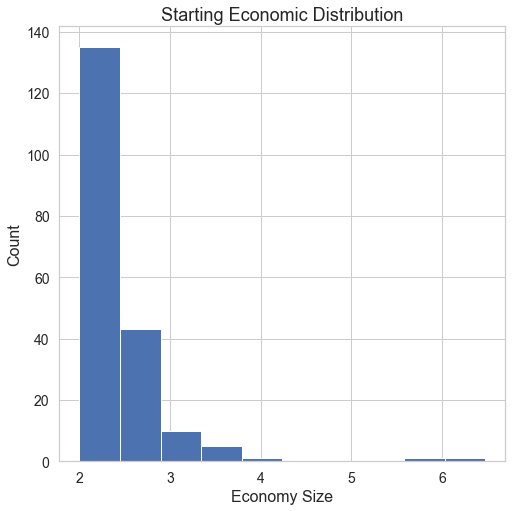
\includegraphics[scale = 0.5]{arming/start_hist.png}
    \caption{Starting arms distribution}
    \label{starthist}
\end{figure}

\noindent Each agent's decision rule is then as follows:

\begin{enumerate}
    \item Survey neighbor arms.
    \item Sum neighbor arms to produce a `threat neighborhood'.\footnote{This type of n-actor threat assessment is never made in models of arming.}
    \item Assess available economic resources after domestic needs are met.
    \item If enough resources remain to balance against the current threat, then the agent increases its arms so that it equals the amount of arms among neighbors.
    \item If there are not enough available resources to meet one's threats, then spend all available resources on arms.
\end{enumerate}

The next series of figures are visualizations of agent arming over time. The first image demonstrates starting arms. Each cell holds one agent and the darker the blue, then the more arms that agent possesses. Curiously, though this shows the model possessing nice emergent properties, the final arms race does not occur where one would expect, given the initial layout.

\begin{figure}
    \centering
    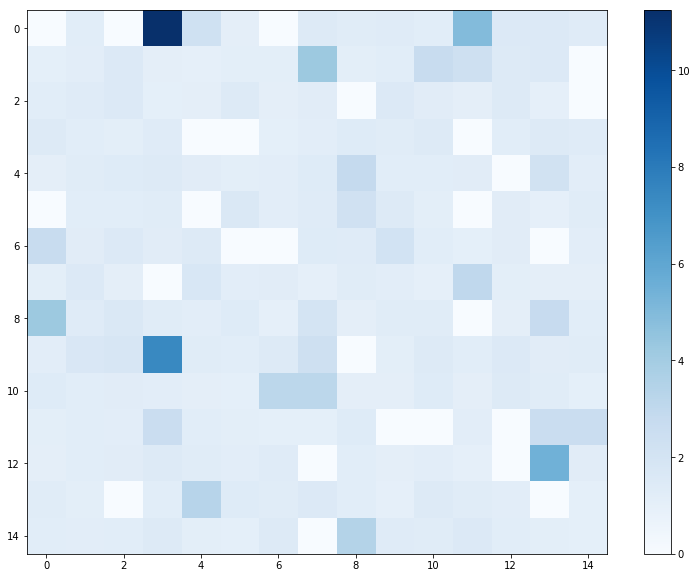
\includegraphics[scale = 0.4]{arming/grid1.png}
    \caption{Initial arms grid}
    \label{grid1}
\end{figure}

Next, I run the model for 200 steps. Each step includes every agent assessing its neighborhood and arming in response to the aggregate threat, insofar as it can economically. The model is set so that agents arm in random order, not simultaneously. We can already see where the model is going here, if we look closely. Some competition is emerging in the center of the grid, but areas on the edges of the grid (which wraps like the world) see no change. In figure \ref{grid3} the model has run for 1000 steps. At this point the writing is on the wall; there is only one arms race in the middle of the grid. But, curiously, the state with the most arms is one that started with relatively low arms.

\begin{figure}
    \centering
    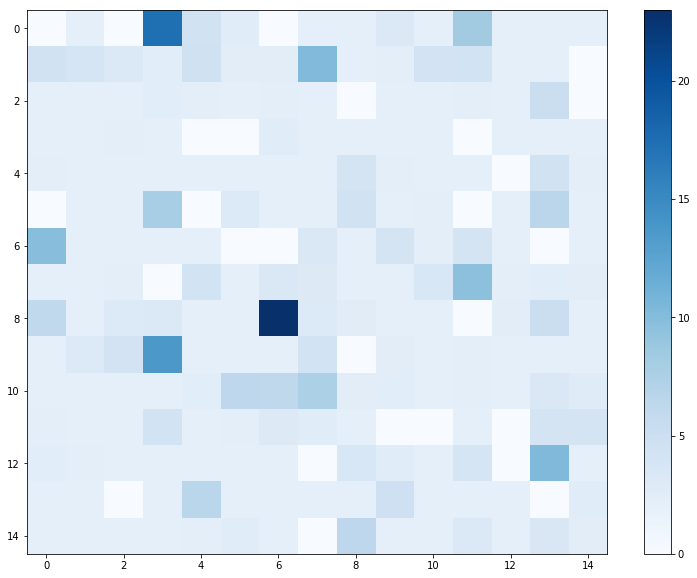
\includegraphics[scale = 0.4]{arming/grid2.png}
    \caption{Arms grid after 200 steps}
    \label{grid2}
\end{figure}


\begin{figure}
    \centering
    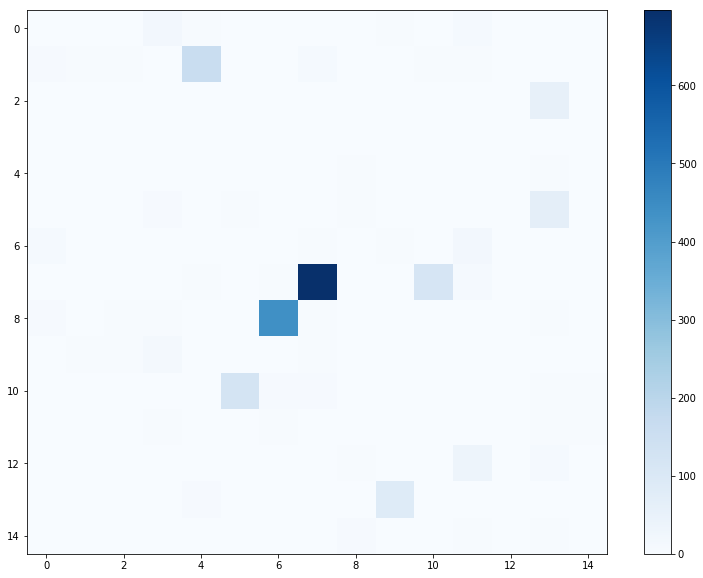
\includegraphics[scale = 0.4]{arming/grid3.png}
    \caption{Arms grid after 1000 steps}
    \label{grid3}
\end{figure}

Last, to let the model run its course, I run it for 5,000 steps. Figure \ref{grid4} includes the final grid and shows a world in which two states are repeatedly arming in response to each other, but all other states have stayed at relatively low arms. This is a promising start in that it very closely mirrors reality. As the final distribution of arms in figure \ref{endhist} demonstrates, the final arms distribution approximates a pareto distribution where two states -- primarily one -- lead all others in arms spending. This is very much the way the world has tended to look throughout history.

\begin{figure}
    \centering
    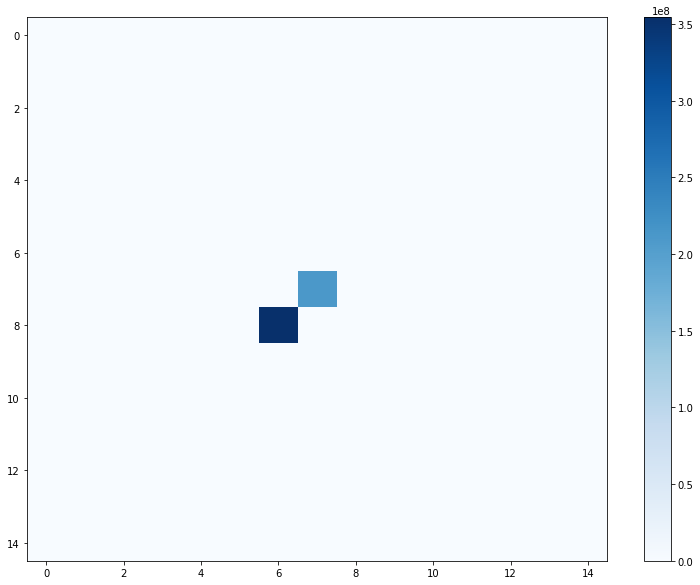
\includegraphics[scale = 0.39]{arming/grid4.png}
    \caption{Arms grid after 5000 steps}
    \label{grid4}
\end{figure}

\begin{figure}
    \centering
    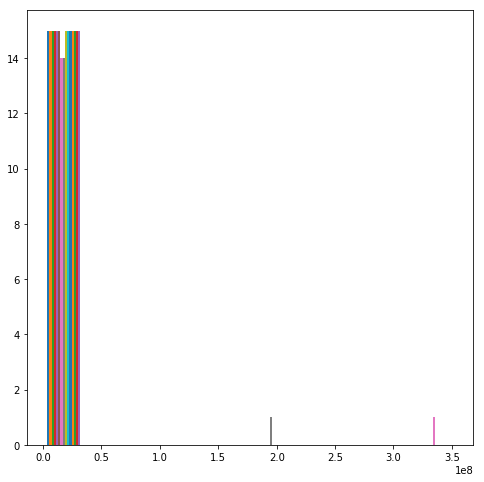
\includegraphics[scale = 0.405]{arming/end_hist.png}
    \caption{Final arms distribution}
    \label{endhist}
\end{figure}

More importantly, seen in this simple framework both the spiral and deterrence models are clearly at play. \textit{This suggests that they are actually more compatible than generally assumed.} For the two states in the center of the grid, a spiral is at hand where each is arming back and forth at each other. Yet for the surrounding states, we see a clear deterrence failure, where they should be arming more to deter the dominant states. And by arming the dominant states do have a strategic advantage over other neighboring states. However, whether or not states find themselves in the deterrence model (failing to balance) or spiral model (costly reciprocal arming) is a function of their strategic environment and domestic constraints. We see agents competing intensely in an arms spiral, states failing to deter, and the competing states gaining great leverage over other neighbors. For all of these situations, states have no incentive to unilaterally deviate given their neighborhood and economic output.

This type of theoretical synthesis is a clear benefit of the agent-based framework. Computer simulation allows for the easy accommodation of an n-player model which would be analytically overwhelming via standard game-theory. And once the outcome emerges from the model it is quite clear that a single strategic framework -- states will balance to meet threats, if it can be afforded -- not only creates a distribution of arms that mirrors reality, but also demonstrates how two seemingly opposed models are very plausibly \textit{separate equilibria in the same overall framework.} Put differently, if we simplify arming to a Prisoner's Dilemma-esque game\footnote{I.e. \citet{jervis1978}}, then the spiral model is (D,D) and deterrence failures are (D,C) and (C, D). But states are `suckered' into (D,C) or (C,D) because they cannot afford to do otherwise.

To be fair, this is far from a final product, and I am clearly oversimplifying. Yet it is quite a powerful result for a first cut: allowing for a guns-butter tradeoff in an n-player model not only generates externally valid trends, it also demonstrates how two classically opposed models can be understood as separate equilibria for a simply utility function when simple parameters vary in realistic ways.


\section{Next Steps}\label{next steps}

Moving forward, there are quite a few steps I need to take before I can make the aforementioned claims credibly. First, the model needs to allow for arming to create bargaining leverage. Arming can confer economic benefits insofar as it gives states leverage in strategically important areas. In this regard, economic growth does not have to be constant, but rather can and should vary based upon how much key strategic territory/issue space a state has occupied via bargaining. Second, I need to think about how to incorporate variables like the offense-defense balance and offense-defense distinguishability into the model. Third, states do not go to war in this model. I am not sure what the decision process behind going to war should look like. It will likely be part of the bargaining process over key territory/issue space, where going to war means the state may be able to take all of the disputed space, rather than bargaining over a proportion of it. Fourth, I have not included any agent learning into this model. Though I would like to do so, I am not sure about how strategic it would be for me publication-wise, because it adds another wrinkle that is foreign to this literature.

Last, incorporating \citet{fearon2018}, I want to use this setup to directly recreate Fearon's model and build upon his theory of the `costs of anarchy'. Beyond testing how prone states are to engage in arms races, a more central question around this whole literature is: how much general military spending do countries need to engage in, given the lack of a world government? In other words, just how costly does anarchy -- understood as the lack of a contract-enforcing central authority in world politics -- have to be? Fearon addresses this through a model of the `war constraint' -- a state's necessary baseline military spending -- and demonstrates how it is a function of the variables just mentioned. Alongside the value of taking his model from 2 states to an n-player world (which is far more credible), he does not touch on the guns-butter tradeoff.

\section{Conclusion}\label{conclusion}

In this paper I have built a simple agent-based model of arms spending. The model reveals that empirical support for the deterrence model over the spiral model is likely a product of states rarely being able to afford arms races. By incorporating a simple guns-butter tradeoff, only a single arms race emerges, despite the model including 225 agents. Moreover, the model's final state includes outcomes that correspond to both the spiral and deterrence model, suggesting that the two models are not actually at odds with each other. Rather they may very well capture separate equilibria for a single utility function, where agents fall into varying equilibria depending on domestic economic pressures and regional arms levels. Last, even from this simple setup, the model is able to closely mirror the actual distribution of military spending worldwide. Though this is a simple first cut, its ability to approximate reality is encouraging.

Moving forward I hope to get this model as close as possible to Fearon's (2018) model, but in an n-player setting with a guns-butter tradeoff. In doing so I can provide a logical next step in the general debate over the `costs of anarchy'. Moreover, in doing so I will be able to better analyze the potential synthesis of the spiral and deterrence models.

\singlespacing

\bibliographystyle{abbrvnat}
\bibliography{prospectus}

\end{document}
